\documentclass[11pt]{article}


\usepackage[top=2cm, bottom=2cm, left=3.5cm, right=3.5cm]{geometry}
\usepackage{hyperref}       % hyperlinks
\usepackage{url}            % simple URL typesetting
\usepackage{booktabs}       % professional-quality tables
\usepackage{microtype}      % microtypography
\usepackage[table, dvipsnames, svgnames]{xcolor}  % colors
\usepackage[outline]{contour}% http://ctan.org/pkg/contour
\usepackage{wrapfig}
\usepackage{graphicx}
\usepackage{bm}
\usepackage{bbm}
\usepackage{multirow}
\usepackage{pifont}
\usepackage{rotating}
\usepackage{tikz}
\usepackage{amsmath}
\usepackage{amsfonts}
\newcommand{\xmark}{\ding{55}}%

\setlength{\tabcolsep}{3.5pt}

\hypersetup{
	colorlinks=true, %set true if you want colored links
	linktoc=all,     %set to all if you want both sections and subsections linked
	linkcolor=black,  %choose some color if you want links to stand out
	citecolor=cyan,
}




\allowdisplaybreaks



\newcommand{\defeq}{\vcentcolon=}
\newcommand{\im}{\operatorname{im}}
\newcommand{\Hom}{{\rm{Hom}}}
\newcommand{\diam}{{\rm{diam}}}
\newcommand{\dom}{\text{dom}}
\newcommand{\ovl}{\overline}
\newcommand{\rr}{\mathbb{R}}
\newcommand{\EE}{\mathcal{E}}
\newcommand{\VV}{\mathcal{V}}
\newcommand{\mystar}{{\fontfamily{lmr}\selectfont$\star$}}
\newcommand{\llangle}{\langle \langle}
\newcommand{\rrangle}{\rangle \rangle}

%bold commands
\newcommand{\xx}{\bm{x}}
\newcommand{\Xx}{\bm{X}}
\newcommand{\Tt}{\bm{T}}
\newcommand{\yy}{\bm{y}}
\newcommand{\ee}{\bm{e}}
\newcommand{\cc}{\bm{c}}
\newcommand{\uu}{\bm{u}}
\newcommand{\vv}{\bm{v}}
\newcommand{\ww}{\bm{w}}
\newcommand{\om}{\bm{\omega}}
\newcommand{\al}{\bm{\alpha}}
\newcommand{\be}{\bm{\beta}}
\newcommand{\si}{\bm{\sigma}}
\newcommand{\ta}{\bm{\tau}}


%calcommand

\newcommand{\mc}{\mathcal}

\DeclareMathOperator*{\argmax}{arg\,max}
\DeclareMathOperator*{\argmin}{arg\,min}

\setlength{\parindent}{0pt}

\author{Simone Manti, AU ID 734894, \texttt{smanti@mpe.au.dk} \\
	Final project for Neural Networks and Deep Learning 2024}

\title{Symbolic Model-Based Reinforcement Learning}



\begin{document}
	\maketitle

\section{Introduction}
This project, highly inspired by \cite{kamienny2022symbolic}, aims to investigate the performance of Symbolic Regression (SR) in Model-Based Reinforcement Learning (MBRL). Indeed, the most common MBRL algorithm choices consist of black-box methods, known to be data-hungry and prone to overfitting when a small amount of data is available. In this project, it has been shown empirically that SR outperforms standard MBRL on simple environments, providing to the user interpretable and simple models.
This study is subdivided as follows:
\begin{itemize}
	\item section 2 introduces the main components of MBRL;
	\item section 3 deals with a short description of SR;
	\item section 4 is dedicated to experiments and implementation details;
	\item finally, section 5 concludes the work with a short discussion. 
\end{itemize}

\section{Model-Based Reinforcement Learning}
Reinforcement Learning (RL), contrarily to standard Supervised Learning, requires a continue interaction with data to update the policy. Usually, model-free RL is employed to optimize the policy, where the agent can only use the data sampled interacting with the real environment. In particular, RL algorithms with high sample complexity are non-manageable in a real-world scenario due to its computational cost. An alternative is presented by the so-called Model-Based Reinforcement Learning (MBRL) \cite{moerland2023model}, where apart from optimizing policy the environment model must be learned. In real-world scenario, having an environment model drastically reduces the complexity of generating new training samples for RL algorithms.
In the following, we briefly overview the main components of MBRL. A more extensive treatment can be found in \cite{moerland2023model, pineda2021mbrl,luo2024survey}. 

MBRL restates the problem as a Markov Decision Process (MDP) \cite{puterman2014}. A MDP is a tuple $\{\mathcal{S}, \mathcal{A}, \mathcal{T}, \mathcal{R}, p(s_0), \gamma\}$, where $\mathcal{S}$ and $\mathcal{A}$ are, respectively, the state and the action space, $\mathcal{T}: \mathcal{S} \times \mathcal{A} \rightarrow p(\mathcal{S})$ is the \textsl{transition function}, $\mathcal{R}: \mathcal{S} \times \mathcal{A} \times \mathcal{S} \rightarrow \rr$ is the \textsl{reward function}, $p(s_0)$ is the initial state distribution and $\gamma \in [0,1]$ is a discount parameter.
A solution to a finite-time MDP consists of a policy $\pi^*: \mathcal{S} \rightarrow \mathcal{A}$ which maximizes the expected sum of rewards, that is
\begin{equation}
	\pi^* = \argmax_{\pi} Q^{\pi}(s,a) = \argmax_{\pi} \mathbb{E}_{\pi, \mathcal{T}}\left[\sum_{k=0}^K \gamma^k r_{t+k} | s_t = s, a_t = a \right], \label{eq: expected_sum_rewards}
\end{equation}

where $s_t \in \mathcal{S}, a_t \in \mathcal{A}, r_t := \mathcal{R}(s_t, a_t, s_{t+1})$.

MBRL approaches repeat the following two steps iteratively:
\begin{enumerate}
	\item collect (or enlarge the current data with) a dataset $\mathcal{D} := \{(s_i, a_i, s_{i+1}, r_i, d_i)\}_{i=1}^N$, where $d_i$ is the termination value indicating the end of the episode, and learn an approximate model $f^*$ of the environment's dynamics fitting $\mathcal{D}$, \textsl{i.e.}
	\begin{equation}
		f^* = \argmax_{f \in \mathcal{F}} \mathbb{E}_{(s_t, a_t, s_{t+1}) \sim \mathcal{D}} \mathcal{L}(s_{t+1}, f(s_t, a_t)),
	\end{equation}
	where $\mathcal{F}$ is a general family of functions (for instance Neural Networks) and $\mathcal{L}$ is a loss function. Note that with the same data reward and termination functions can be learned reward as well;
	\item simulate the transition with the learned model $f^*$ and optimize the policy maximizing the expected sum of rewards like in \eqref{eq: expected_sum_rewards}.
\end{enumerate}

\section{Symbolic Regression}
SR consists of finding a mathematical expressions that best fits a given dataset without assuming a particular structure of the expression. 
In our case, SR is handled with Genetic Programming (GP) \cite{koza1994genetic, o2009riccardo}. GP is an evolutionary strategy that explores a space of candidate models/functions by iteratively updating an initial population through genetic operations. A candidate model is also called \textsl{individual} and can be easily represented by a tree, in which each node is either a \textsl{primitive} (\textsl{i.e.} an operator) or a \textsl{terminal} (\textsl{i.e.} a variable or constant).
\paragraph{Initialization} The population is typically initialized randomly. Some well-known techniques are the \textsl{full} and the \textsl{grow} method (see Section 2.1 in \cite{o2009riccardo}), and a combination of those gives rise to \textsl{ramped half and half}. Each of them assumes that the starting population contains individuals that do not exceed a fixed maximum depth.

\paragraph{Selection} Usually genetic operations are performed on individuals that are selected based on fitness, \textsl{i.e.} that are ``probably good''. One way to do so is \textsl{tournament selection}. This consists of performing a tournament for each $k$ (tournament size) individuals, competing in terms of their fitnesses. The higher the score in these tournaments, the higher the probability for these individuals to be chosen. In our method, $k=2$ and we assign a non-zero probability to pick the loser instead of the winner in each tournament. This is calibrated in the hyperparameter selection phase. 

\paragraph{Crossover and Mutation} Genetic operations consists of \textsl{crossover} and \textsl{mutation}. The most common crossover used is the \textsl{subtree crossover} (or \textsl{one-point crossover}): given two parent trees, a random subtree and a crossover point are chosen for both; then, two new trees are generated, named \textsl{offsprings}, replacing the subtree rooted in the first parent with the one in the second parent and vice-versa.
Instead, the most common mutation creates an offspring for a given parent tree by replacing a (randomly chosen) subtree with a newly generated subtree. 

\section{Experiments and implementations details}
SR for MBRL performance is assessed through 2 different experiments, inspired by \cite{kamienny2022symbolic}. In both of them, a comparison with MBRL through Neural Networks (NN) is made. The MBRL algorithm chosen for SR and NN is the Probablistic Ensembles with Trajectory Sampling (PETS) \cite{chua2018deep}, implemented with MBRL-lib \cite{pineda2021mbrl} for NN and Operon \cite{burlacu2020operon} for SR. The action optimizer used is the Cross-Entropy Method (CEM) \cite{de2005tutorial}.
The implementation of this project is open-source and it is accessible through a public GitHub repository \cite{???} \textcolor{red}{link github repo}.


\subsection{Simple 1-dimensional MDP}
\label{sec: simple_1_dmdp}
The following simple 1-dimensional MDP, with episode length 10, is considered
\begin{align}
	&s_{t+1} := s_t + a_t, \label{eq: simple_1dmpd_dynamics}\\ 
	&r_t := \cos(2\pi s_{t+1})\exp(|s_{t+1}|/3). \label{eq: simple_1dmpd_reward}
\end{align}

In this case, the goal is learning both the dynamics eq.~\eqref{eq: simple_1dmpd_dynamics} and the reward function eq.~\eqref{eq: simple_1dmpd_reward}. The training (500) and validation (100) transitions were collected by sampling uniformly in the action space [-1,1] (random policy). A single run of PETS was used for both SR and NN.

\paragraph{SR hyperparameters} The following hyperparameters are used: 10 optimizer iterations, population size 5000, 10000 generations, \texttt{add,sub,mul,div,constant,variable,} \texttt{sin,exp,abs} as allowed symbols and 32 threads. Note that to complicate the problem \texttt{cos} is not in the primitive set.

\paragraph{NN hyperparameters} A standard Multi-Layer Perceptron (MLP) is considered with the following hyperparameters: 4 hidden layers with 200 nodes each, SiLU activation function, Adam optimizer with 2000 epochs, batch size 256, patience epochs 25, learning rate $7.5e-4$ and weight decay $3e-5$.

\paragraph{Action Optimizer} CEM is used with planning horizon 3, 10 iterations, elite ratio 0.1, population size 1000, alpha 0.1 and clipped normal action distribution.

\paragraph{Results} Figure~\ref{fig: simple_1dmdp} demonstrates that SR learned solution generalizes better outside the training region, while the NN model overfits in the training distribution. SR learned the following models (rounded to the first $3$ decimal digits):
\begin{align}
	&s_{t+1} = 1.0s_t + 1.0a_t, \label{eq: sr_simple_1dmdp_dynamics}\\
	&r_t = 1.0\exp(|0.333s_{t+1}|)\sin(6.283s_{t+1} - \left|-0.023 s_t + \sin(0.023 s_t) + 1.571\right|).\label{eq: sr_simple_1dmdp_reward}
\end{align}

Note that eq.~\eqref{eq: simple_1dmpd_dynamics} coincides with eq.~\eqref{eq: simple_1dmpd_dynamics}, while eq.~\eqref{eq: sr_simple_1dmdp_reward} is slightly different than eq.~\eqref{eq: simple_1dmpd_reward}. However, the first of the two factors matches completely with the ground truth, while the latter is approximately $\sin(2\pi s_{t+1} + 1.571)$ using that $6.283\approx 2\pi$ and that $sin(x) \approx x$ for $x>0$ sufficiently small. A similar model for the reward function was also found in the original paper \cite{kamienny2022symbolic}.

\begin{figure}
	\centering
	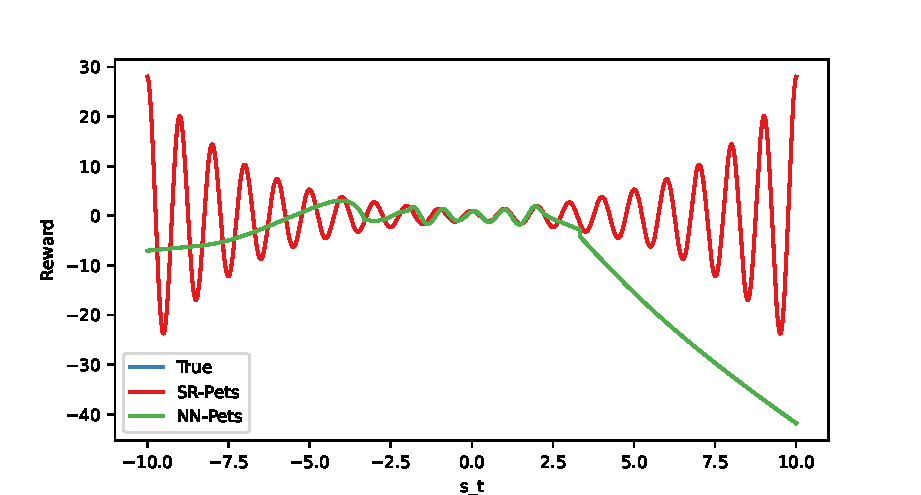
\includegraphics{simple1dmdp_pets.pdf}
	\caption{Reward function, evaluated with $a_t=0$, predicted by the learned models}
	\label{fig: simple_1dmdp}
\end{figure}

\subsection{Cartpole}
The continuous Cartpole \cite{brockman2016openai, todorov2012mujoco} is considered, where the agent's action $a$ influences the system's state based on the following equations \cite{florian2007correct}:

\begin{align}
	&\ddot{\theta} = \frac{g\sin(\theta) + \cos(\theta)\left(\frac{-K_{\rm mag} a - m_p l \dot{\theta}^2\sin(\theta)}{m_c + m_p}\right)}{l\left(\frac{4}{3} - \frac{m_p\cos^2(\theta)}{m_c+m_p}\right)}, \label{eq: cartpole_theta}\\
	& \ddot{x} = \frac{K_{\rm mag} a + m_pl(\dot{\theta}^2\sin(\theta) - \ddot{\theta}\cos(\theta))}{m_c + m_p} \label{eq: cartpole_x},
\end{align}

where $g,K_{\rm mag}, m_p, m_c$ and $l$ are constants. The agent state is $s_t := (x_t, \theta_t, \dot{x}_t, \dot{\theta}_t)$, and the task is purely related to dynamics modeling, since both termination and reward functions are known to the agent \cite{pineda2021mbrl, chua2018deep}. 

The initial training (10) and validation (40) transition were collected using a random policy. Then, PETS was run for 10 iterations, and in each of those 10 transitions using the current policy. This procedure was repeated 3 times and the results were averaged accordingly.

\paragraph{SR hyperparameters} As in \ref{sec: simple_1_dmdp} but with allowed symbols \texttt{add,sub,mul,div,constant,} \texttt{variable,sin,cos,square}.

\paragraph{NN hyperparameters} As in \ref{sec: simple_1_dmdp}.

\paragraph{Action Optimizer} CEM is used with planning horizon 15, 5 iterations, elite ratio 0.1, population size 350, alpha 0.1.

\paragraph{Results} Also in this case SR outperforms NN, being able to learn a good controller using only 10 training transitions (Figure~\ref{fig: cartpole}A). The SR models found at the end of a random PETS episode are the following

\begin{align}
	&x_{t+1} = 1.0x_t + 0.020\dot{x}_t,\\
	&\theta_{t+1}=(\theta_t - 0.014\dot{x}_t + 0.195a_t)\cos(0.228\dot{x}_t),\\
	&\dot{x}_{t+1} = 1.0\dot{x}_t + 0.020 \dot{\theta}_t,\\
	&\dot{\theta}_{t+1} = 0.315\dot{x}_t +1.0\dot{\theta}_t - 3.87a_t\cos(0.311\dot{x}_t) + 3.577a_t - 0.000.
\end{align}

Even though we can recognize some similarities with the ground-truth eq.~\eqref{eq: cartpole_theta}-\eqref{eq: cartpole_x}, \textsl{e.g.} the time-discretization interval 0.02, the SR models are slightly different. This can be explained by the fact that a good candidate can have large validation MSE (Figure~\ref{fig: cartpole}B).

\begin{figure}
	\centering
	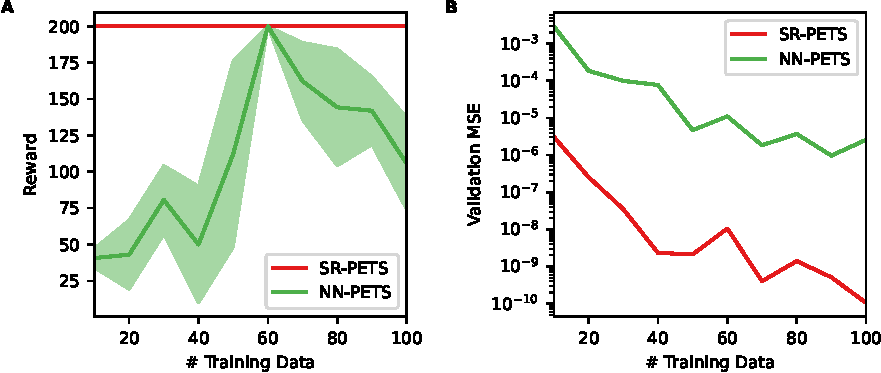
\includegraphics{cartpole.pdf}
	\caption{Evolution of cumulative reward (A) and validation MSE (B) as the number of training transitions increases. The results were averaged over 3 episodes with 3 random seeds.}
	\label{fig: cartpole}
\end{figure}


\section{Conclusion and discussion}
This project demonstrates that SR-based MBRL can be more effective than standard MBRL in simple yet challenging environments, discovering models with many less parameters and better generalization capabilities. Also, interpretability of SR models can help scientists to manage and explain more easily the learned dynamics/rewards.

\bibliographystyle{ieeetr}
\begin{thebibliography}{10}
	\bibitem{kamienny2022symbolic}
	P.A.~Kamienny, S.~Lamprier, ``Symbolic-Model-Based Reinforcement Learning''.
	{\em NeurIPS 2022 AI for Science: Progress and Promises}, 2022.
	
	\bibitem{puterman2014}
	M. L.~Puterman, ``Markov Decision Processes: Discrete Stochastic Dynamic Pro-
	gramming.'' {\em John Wiley and sons}, 2014.
	
	\bibitem{moerland2023model}
	T.M.~Moerland, J.~Broekens, A.~Plaat, C.M.~Jonker, ``Model-based Reinforcement Learning: A Survey''. {\em Foundations and Trends in Machine Learning}, 2023.
	
	\bibitem{pineda2021mbrl}
	L.~Pineda, B.~Amos, A.~Zhang, N.O~Lambert, R.~Calandra, ``Mbrl-lib: A Modular Library for Model-Based Reinforcement Learning''. {\em arXiv preprint arXiv:2104.10159}, 2021.
	
	\bibitem{luo2024survey}
	F.~Luo, T.~Xu, H.~Lai, X.~Chen, W.~Zhang, Y.~Yu, ``A Survey on Model-Based Reinforcement Learning''. {\em Science China Information Sciences}, 2024.
	
	\bibitem{koza1994genetic}
	J.R.~Koza, ``Genetic programming as a means for programming computers by natural selection'', 
	{\em Statistics and Computing}, 1994.
	
	\bibitem{o2009riccardo}
	R.~Poli et al., ``A Field Guide to Genetic Programming''.
	\newblock Published via \texttt{http://lulu.com} and freely available at \texttt{http://www.gp-field-guide.org.uk}, 2008.
	
	\bibitem{barto1983neuronlike}
	A.G.~Barto, R.S.~Sutton,C.W.~Anderson, ``Neuronlike adaptive elements that can solve difficult learning control problems''. {\em IEEE transactions on systems, man, and cybernetics}, 1983.
	
	\bibitem{florian2007correct}
	R.V~Florian, ``Correct equations for the dynamics of the cart-pole system''. {\em Center for Cognitive and Neural Studies (Coneural)}, 2007.
	
	\bibitem{brockman2016openai}
	G.~Brockman, V.~Cheung, L.~Pettersson, J.~Schneider, J.~Schulman, J.~Tang, W.~Zaremba, ``Openai gym''. {\em arXiv preprint arXiv:1606.01540}, 2016.
	
	\bibitem{todorov2012mujoco}
	E.~Todorov, T.~Erez, Y.~Tassa, ``Mujoco: A physics engine for model-based control''. {\em IEEE/RSJ International Conference on Intelligent Robots and Systems}, 2012
	
	\bibitem{chua2018deep}
	K.~Chua, R.~Calandra, R.~McAllister, Sergey.~Levine, ``Deep reinforcement learning in a handful of trials using probabilistic dynamics models''. {\em Advances in Neural Information Processing Systems}, 2018.
	
	\bibitem{burlacu2020operon}
	B.~Burlacu, G.~Kronberger, M.~Kommenda, ``Operon C++: An efficient genetic programming framework for symbolic regression". {\em Proceedings of the 2020 Genetic and Evolutionary Computation Conference Companion, GECCO}  2020.
	
	\bibitem{de2005tutorial}
	P.T.~De Boer, D.P.~Kroese, S.~Mannor, R.Y.~Rubinstein, ``A tutorial on the cross-entropy method". {\em Annals of operations research}, 2005.
	
\end{thebibliography}
\end{document}